% 4,6 : Paul
% 7,8 : Jo'
% 9,10,11,13: Anthony

\documentclass{article}

\usepackage{a4}
\usepackage{amsmath}
\usepackage{amsfonts}
\usepackage{amssymb}
\usepackage{float}
\usepackage[utf8]{inputenc}
\usepackage[T1]{fontenc}

\usepackage{framed}

\usepackage{graphicx}
\usepackage{caption}
\usepackage{subcaption}
\usepackage{wrapfig}

\usepackage{geometry}


\usepackage{fullpage,graphicx}
\usepackage{rotating}

\usepackage{multirow}

%\setlength{\hoffset}{-18pt}
\setlength{\oddsidemargin}{0cm}     % Marge gauche sur pages impaires
\setlength{\evensidemargin}{0cm}    % Marge gauche sur pages paires
\setlength{\marginparwidth}{54pt}   % Largeur de note dans la marge
\setlength{\textwidth}{17cm}       % Largeur de la zone de texte (17cm)
\setlength{\marginparsep}{7pt}      % Séparation de la marge
\setlength{\topmargin}{-1cm}         % Pas de marge en haut
\setlength{\headheight}{0cm}       % Haut de page
\setlength{\headsep}{10pt}          % Entre le haut de page et le texte
\setlength{\footskip}{27pt}         % Bas de page + séparation
\setlength{\textheight}{23cm}      % Hauteur de la zone de texte (25cm)

\setlength{\parskip}{1ex}
\setlength{\parindent}{1cm}

%\setlength{\topsep}{500pt}
\setlength{\abovecaptionskip}{0.1cm}
\setlength{\belowcaptionskip}{0.5cm}



\newlength{\leftbarwidth}
\setlength{\leftbarwidth}{3pt}
\newlength{\leftbarsep}
\setlength{\leftbarsep}{10pt}
\newlength{\leftbarmargin}
\setlength{\leftbarmargin}{0pt}
\newlength{\defaultparindent}
\setlength{\defaultparindent}{\parindent}


\renewenvironment{leftbar}{%
    \def\FrameCommand{\hspace{\leftbarmargin} \vrule width \leftbarwidth \relax\hspace{\leftbarsep}}%
    \MakeFramed {\advance \hsize -\width \FrameRestore }%
}{%
    \endMakeFramed
}


%\newenvironment{defx}{\noindent \\ \textbf{Definition:} \vspace{-11pt} \begin{leftbar} \vspace{4pt}}{\end{leftbar}}
%\newenvironment{propx}{\noindent \\ \textbf{Proposition:} \vspace{-11pt} \begin{framed}}{\end{framed}}

\newenvironment{defx}{
\setlength{\leftbarwidth}{3pt} 
\setlength{\leftbarmargin}{-2pt} 
\setlength{\leftbarsep}{10pt} 
\begin{leftbar}}{\end{leftbar}}
\newenvironment{propx}{\begin{framed}}{\end{framed}}

\newenvironment{demox}{\footnotesize \noindent \textit{Demo:}  \vspace{-9pt} 
\setlength{\leftbarwidth}{1pt} 
\setlength{\leftbarmargin}{5pt}
\setlength{\leftbarsep}{3pt} 
\setlength{\parindent}{7pt}

\begin{leftbar}}{\end{leftbar}
\setlength{\parindent}{\defaultparindent}
\normalsize}



\newenvironment{deft}[1]{\noindent \\ \textbf{\textsc{#1}} \vspace{-11pt} \setlength{\leftbarwidth}{3pt} 
\setlength{\leftbarmargin}{-2pt} 
\setlength{\leftbarsep}{10pt} 
\begin{leftbar} \vspace{4pt}}{\end{leftbar}}
\newenvironment{propt}[1]{\noindent \\ \textbf{\textsc{#1}} \vspace{-11pt} \begin{framed}}{ \end{framed}}


\newenvironment{algot}[1]{\noindent \\ \textbf{\textsc{#1}} \par \nobreak \vspace{1pt}\hrule\vspace{0pt} \setlength{\parindent}{0cm} \ttfamily} {\normalfont \setlength{\parindent}{\defaultparindent} \par \nobreak \vspace{4pt}\hrule\vspace{15pt}}

\newenvironment{algox}{\noindent \\  \par \nobreak \vspace{1pt}\hrule\vspace{0pt} \setlength{\parindent}{0cm} \ttfamily} {\normalfont \setlength{\parindent}{\defaultparindent} \par \nobreak \vspace{4pt}\hrule\vspace{15pt}}

%\newenvironment{algot}[1]{\noindent \\ \textbf{\textsc{#1}} \par \nobreak \vspace{1pt}\hrule\vspace{0pt} \setlength{\parindent}{0cm} \ttfamily \begin{tabbing} ~~~~\=~~~~\=~~~~\=~~~~\=~~~~\=~~~~\=~~~~} {\end{tabbing} \normalfont \setlength{\parindent}{\defaultparindent} \par \nobreak \vspace{4pt}\hrule \\}

\newcommand{\comment}[1]{\hfill// #1}

\newcommand{\bbB}{\mathbb{B}}
\newcommand{\bbN}{\mathbb{N}}
\newcommand{\bbZ}{\mathbb{Z}}
\newcommand{\bbR}{\mathbb{R}}

\newcommand{\tb}{.~~~~}

%\newcommand{\exsubpart}[1]{\subsection*{#1)}\\ }
\newcommand{\exsubpart}[1]{\subsection*{#1)} \vspace{-51pt} ~\\}

\newcommand{\info}[1]{\small{\textit{(#1)}}}



\graphicspath{{./Images/}}

\begin{document}

\noindent {\fontsize{20}{20}\selectfont \noindent \textbf{Laboratoire d'électronique~:}}

\noindent {\fontsize{30}{30}\selectfont \noindent \textbf{Convertisseurs A/N et N/A}}

\vspace{5pt}\hrule\vspace{2pt}

\noindent {\Large \textbf{\textsc{Masur} Jonathan}\hfill\textbf{\textsc{Graignic} Anthony}\hfill \textbf{\textsc{Gosselin} Paul}}

\vspace{20pt}


% Return loss

% 4.2.2
% Désadaptation d'impédance
% Voir HF-VHF : 2.16, 3.22





\section{L'amplificateur accordé}

\subsection{Description}

On considère l'amplificateur accordé décrit Fig.~\ref{schem6}.

\begin{figure}[h!]
	\centering
	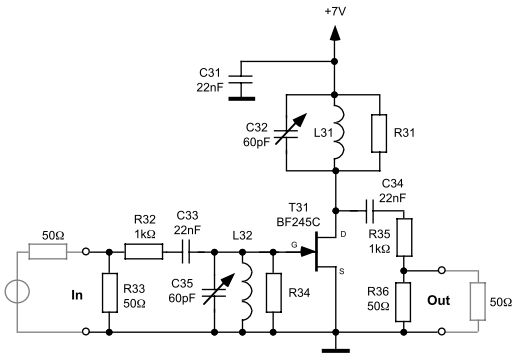
\includegraphics[width=.7\textwidth]{schem6}
	\caption{}
	\label{schem6}
\end{figure}


\subsection{Questions et calculs}

\exsubpart{1}

Les deux circuits résonnants sont couplés via un couplage actif.

\exsubpart{2}

On couple deux filtres d'ordre 1, formant ainsi un filtre d'ordre 2.

Si le facteur de qualité de chacun des circuits résonants est le même, on obtient donc un facteur de qualité global de~:
\begin{equation*}
Q_{tot} = \frac{1}{\sqrt{2^{1/2}-1}}Q = 1,554 Q
\end{equation*}


\exsubpart{3}

Les condensateurs $C_{33}$ et $C_{34}$ permettent uniquement de couper de très basses fréquences, hors de notre domaine d'intérêt. On peut donc les ignorer.

Les filtres restants en amont et en aval du JFET sont tout deux constitués d'une inductance et d'une capacité en parallèle, liées à une tension de référence. Ce sont deux passe-bande d'ordre 2~: l'ordre est de 1 de chaque côté de la fréquence de résonance, donnant donc lieu à des pentes de $\pm$20 dB/décade de part et d'autre de cette fréquence.

En couplant ces deux filtres, on obtient donc un filtre passe-bande d'ordre total 4. On trouve de part et d'autre de la fréquence de résonance $f_0$ un ordre 2, soit des pentes de +20 dB/décade et -20 dB/décade respectivement en-dessous et au-dessus de $f_0$.


\exsubpart{4}

Afin d'obtenir une bande passante à -3dB s'étendant de $f_1 = $13 MHz à $f_2 = $15 MHz, le facteur de qualité total doit être de~:
\begin{equation*}
Q_{tot} = \frac{f_0}{f_2-f_1}
\end{equation*}
avec $f_0 = $14 MHz, soit~:
\begin{equation*}
Q_{tot} = 7
\end{equation*}

Cela correspond pour chaque circuit résonant à un facteur de qualité de~:
\begin{equation*}
Q = \sqrt{2^{1/2}-1}~Q_{tot} = 4,505
\end{equation*}


%Toutefois, on prendra $R_{31}=R_{34}=\infty$~: en effet, ces résistances on juste pour but de diminuer les facteurs de qualité des filtres situés en amont et en aval du JFET.
% L31 = L32 = 2.2 uH


% 5) On saute...





\section{L'oscillateur à quartz}

\subsection{Description}

La réaction positive s'effectue par le condensateur parasite $C_{bc}$ qui se trouve entre le collecteur et la base du transistor.
\begin{center}
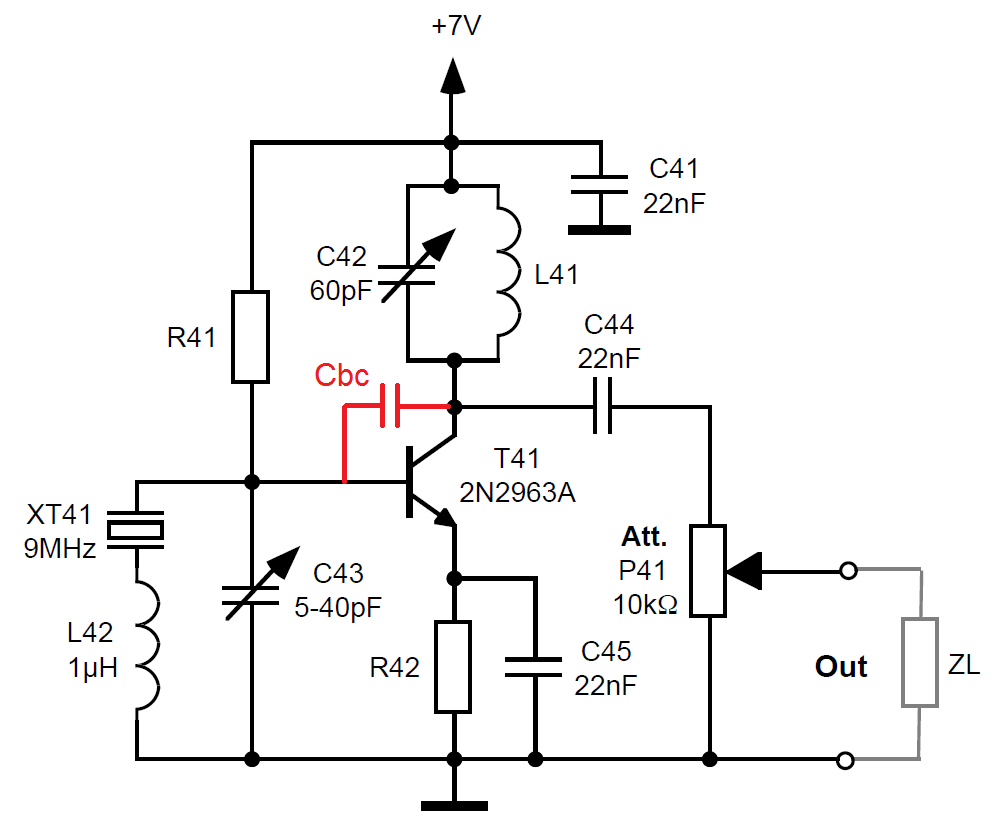
\includegraphics[width = 0.7\linewidth]{shema_oscillateur.png}
\end{center}
L'oscillateur est de type Colpitts, c'est à dire que la réaction positive est réalisée par un diviseur capacitif.\\
Si on considère le schéma petits signaux (suppression des composantes continues servant à polariser le transistor) on obtient le schéma suivant :
\begin{center}
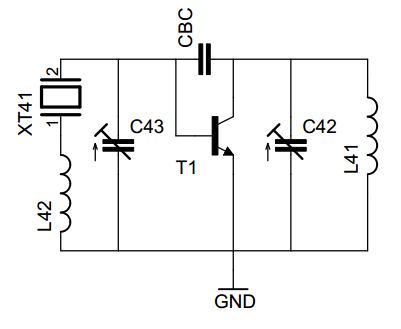
\includegraphics[width=0.4\linewidth]{shema_petit_signaux_oscillateur.png}
\end{center}
On voit alors que le circuit de charge est un filtre passe-bande formé par $L_{41}$ et $C_{42}$. Les fréquences seront toutes atténuées, sauf celles proches de la fréquence de résonance $f_0$, où $f_0 = \frac{1}{2 \pi \cdot \sqrt{L_{41} \cdot C_{42}}}$.\\
En admettant qu'à l'enclenchement du circuit, il y a du bruit blanc sur la base du transistor, ce bruit blanc inclut toutes les fréquences y compris $f_0$. Il ne restera plus que $f_0$ à la sortie, qui sera alors ré-injectée dans la base par le diviseur formé par $C_{BC}$ et $C_{43}$.\\
La condition pour que l'oscillation démarre est que le gain du transistor doit être plus grand que l'atténuation du diviseur captatif. La branche avec le quartz n'est pas nécessaire pour l'apparition d'une oscillation. Cependant elle sert a sélectionner une fréquence particulière de façons plus précise.

En effet, le quartz agit comme un filtre supplémentaire, et son facteur de qualité Q est très largement plus élevé que celui d'un filtre à composant LC (qui présentent des imperfections électromécaniques).\\

Le quartz peut être modélisé de la façon suivante :\footnote{Source : $www.acedim.com/Formatronic/Electro_2/oscillateur/lequartz.html$}
\begin{center}
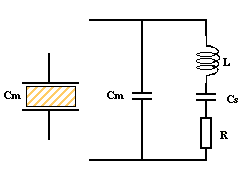
\includegraphics[width=0.4\linewidth]{modele_quartz.png}
\end{center}
Il a alors deux fréquences de résonances : fp$=\frac{1}{2\pi \cdot L_s \cdot C_s}$ et fs$=\frac{1}{2\pi \cdot L_s \cdot C_{eq}}$, où $C_{eq} = \frac{1}{\frac{1}{C_s} + \frac{1}{C_m}}$. Ces deux fréquences sont en général très proches l'une de l'autre.\\
Le quartz est capacitif sur toutes les plages de fréquences sauf dans la bande très étroite qui se trouve entre fp et fs \footnote{Source : $http://www.acedim.com/Formatronic/Electro_2/oscillateur/oscilaquartz.html$}:
\begin{center}
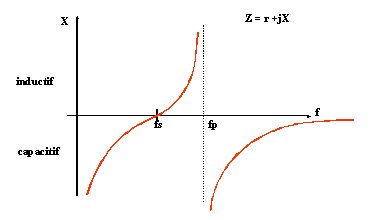
\includegraphics[width=0.4\linewidth]{impedence_quartz.png}
\end{center}

Le quartz a un comportement inductif à la fréquence d'oscillation, qui est donc toujours comprise entre fp et fs.\\

Il est nécessaire que le résonateur $L_{41}$ et $C_{42}$ soit accordé à une fréquence très proche de celle du quartz, sinon les deux filtres vont s'annuler réciproquement et il n'y aura pas d'oscillations.\\

Le condensateur $C_{42}$ a peu d'influence sur la fréquence de sortie. En effet, changer son réglage changera $f_0$, mais le filtre réalisé par le Quartz ayant un facteur de qualité beaucoup plus grand, c'est lui qui sera déterminant pour la fréquence des oscillations. Si $C_{42}$ est mal réglé, nous aurons simplement une atténuation de l'amplitude des oscillations, ou carrément un arrêt de l'oscillateur.\\
En revanche le réglage de $C_{43}$ vient affecter directement le quartz, et va donc avoir un effet direct sur la fréquence d'oscillation.\\
Le fait de brancher une charge à la sortie ve diminuer le facteur de qualité du résonateur $L_{41}$ et $C_{42}$. Cela va donc affecter le rapport de force entre ce filtre et le quartz. Plus la résistance de charge est faible, plus le facteur de qualité baisse donc plus la fréquence sera proche de celle du Quartz, ce qui est l'idéal.

\subsection{Dimentionement de la polarisation}
On fait une analyze en grand signaux, c'est à dire que toutes les inductances sont des court-circuits, et les capacités ainsi que le quartz sont circuits ouverts.\\
Le courant de repos Ic de $1mA$ doit circuler dans le collecteur et l'émetteur du transistor. On désire avoir 1V sur l'émetteur, d'où la valeur de $R_{42}$ :
\begin{center}
$R_{42} = \frac{U_e}{Ic} = \frac{1V}{1mA} = 1k\Omega$
\end{center}
Puis, le courant circulant dans la base du transistor, et donc dans $R_{41}$ est $\beta$ fois plus petit que Ic.\\
Le facteur $\beta$ varie fortement avec la température et d'un transistor à l'autre, cependant on peut pour ce transistor estimer que $\beta \simeq 100$ d'où :
\begin{center}
$Ib = \frac{Ic}{\beta} = \frac{1mA}{100} = 10\mu A$
\end{center}
La tension entre la base et l'émetteur est identique à celle d'une diode en conduction $Uj \simeq 0.7V$, d'où :
\begin{center}
$R_{41} = \frac{U_{R41}}{I_{R41}} = \frac{Vcc - Ub}{Ib} = \frac{Vcc - Uj - Ue}{Ib} = \frac{7V - 0.7V - 1V}{1mA} = 530k\Omega$
\end{center}
Nous prenons donc une valeur normalisée de $470k\Omega$, arrondi en dessous car il vaut mieux que Ib et Ic soient un peu plus grand que prévu (transistor conduit mieux) que l'inverse.\\

La sortie, qui se trouve sur le collecteur du transistor, peut osciller librement entre la tension d'émetteur, qui est de 1V, et la tension d'alimentation, qui est de $7V$. Il est donc possible d'avoir jusqu'à 6V d'amplitude en sortie.\\

\subsection{Calcul de l'inductance}
La fréqunce de résonance de la charge au collecteur est donnée par :
\begin{center}
$f_0 = \frac{1}{2\pi \sqrt{L_{41} \cdot C_{42}}}
\Rightarrow
L_{41} = \frac{1}{(2\pi f_0)^2 \cdot C_{42}} = \frac{1}{(2\pi \cdot 9 \cdot 10^6)^2 \cdot 60 \cdot 10^{-12}} = 5.22 \mu H$
\end{center}
On a utilisé la valeur normalisée la plus proche, c'est à dire $5.6 \mu H$

\subsection{Mesures}
Spectre de sortie autour de la fondamentale à 9MHz :\\
\begin{center}
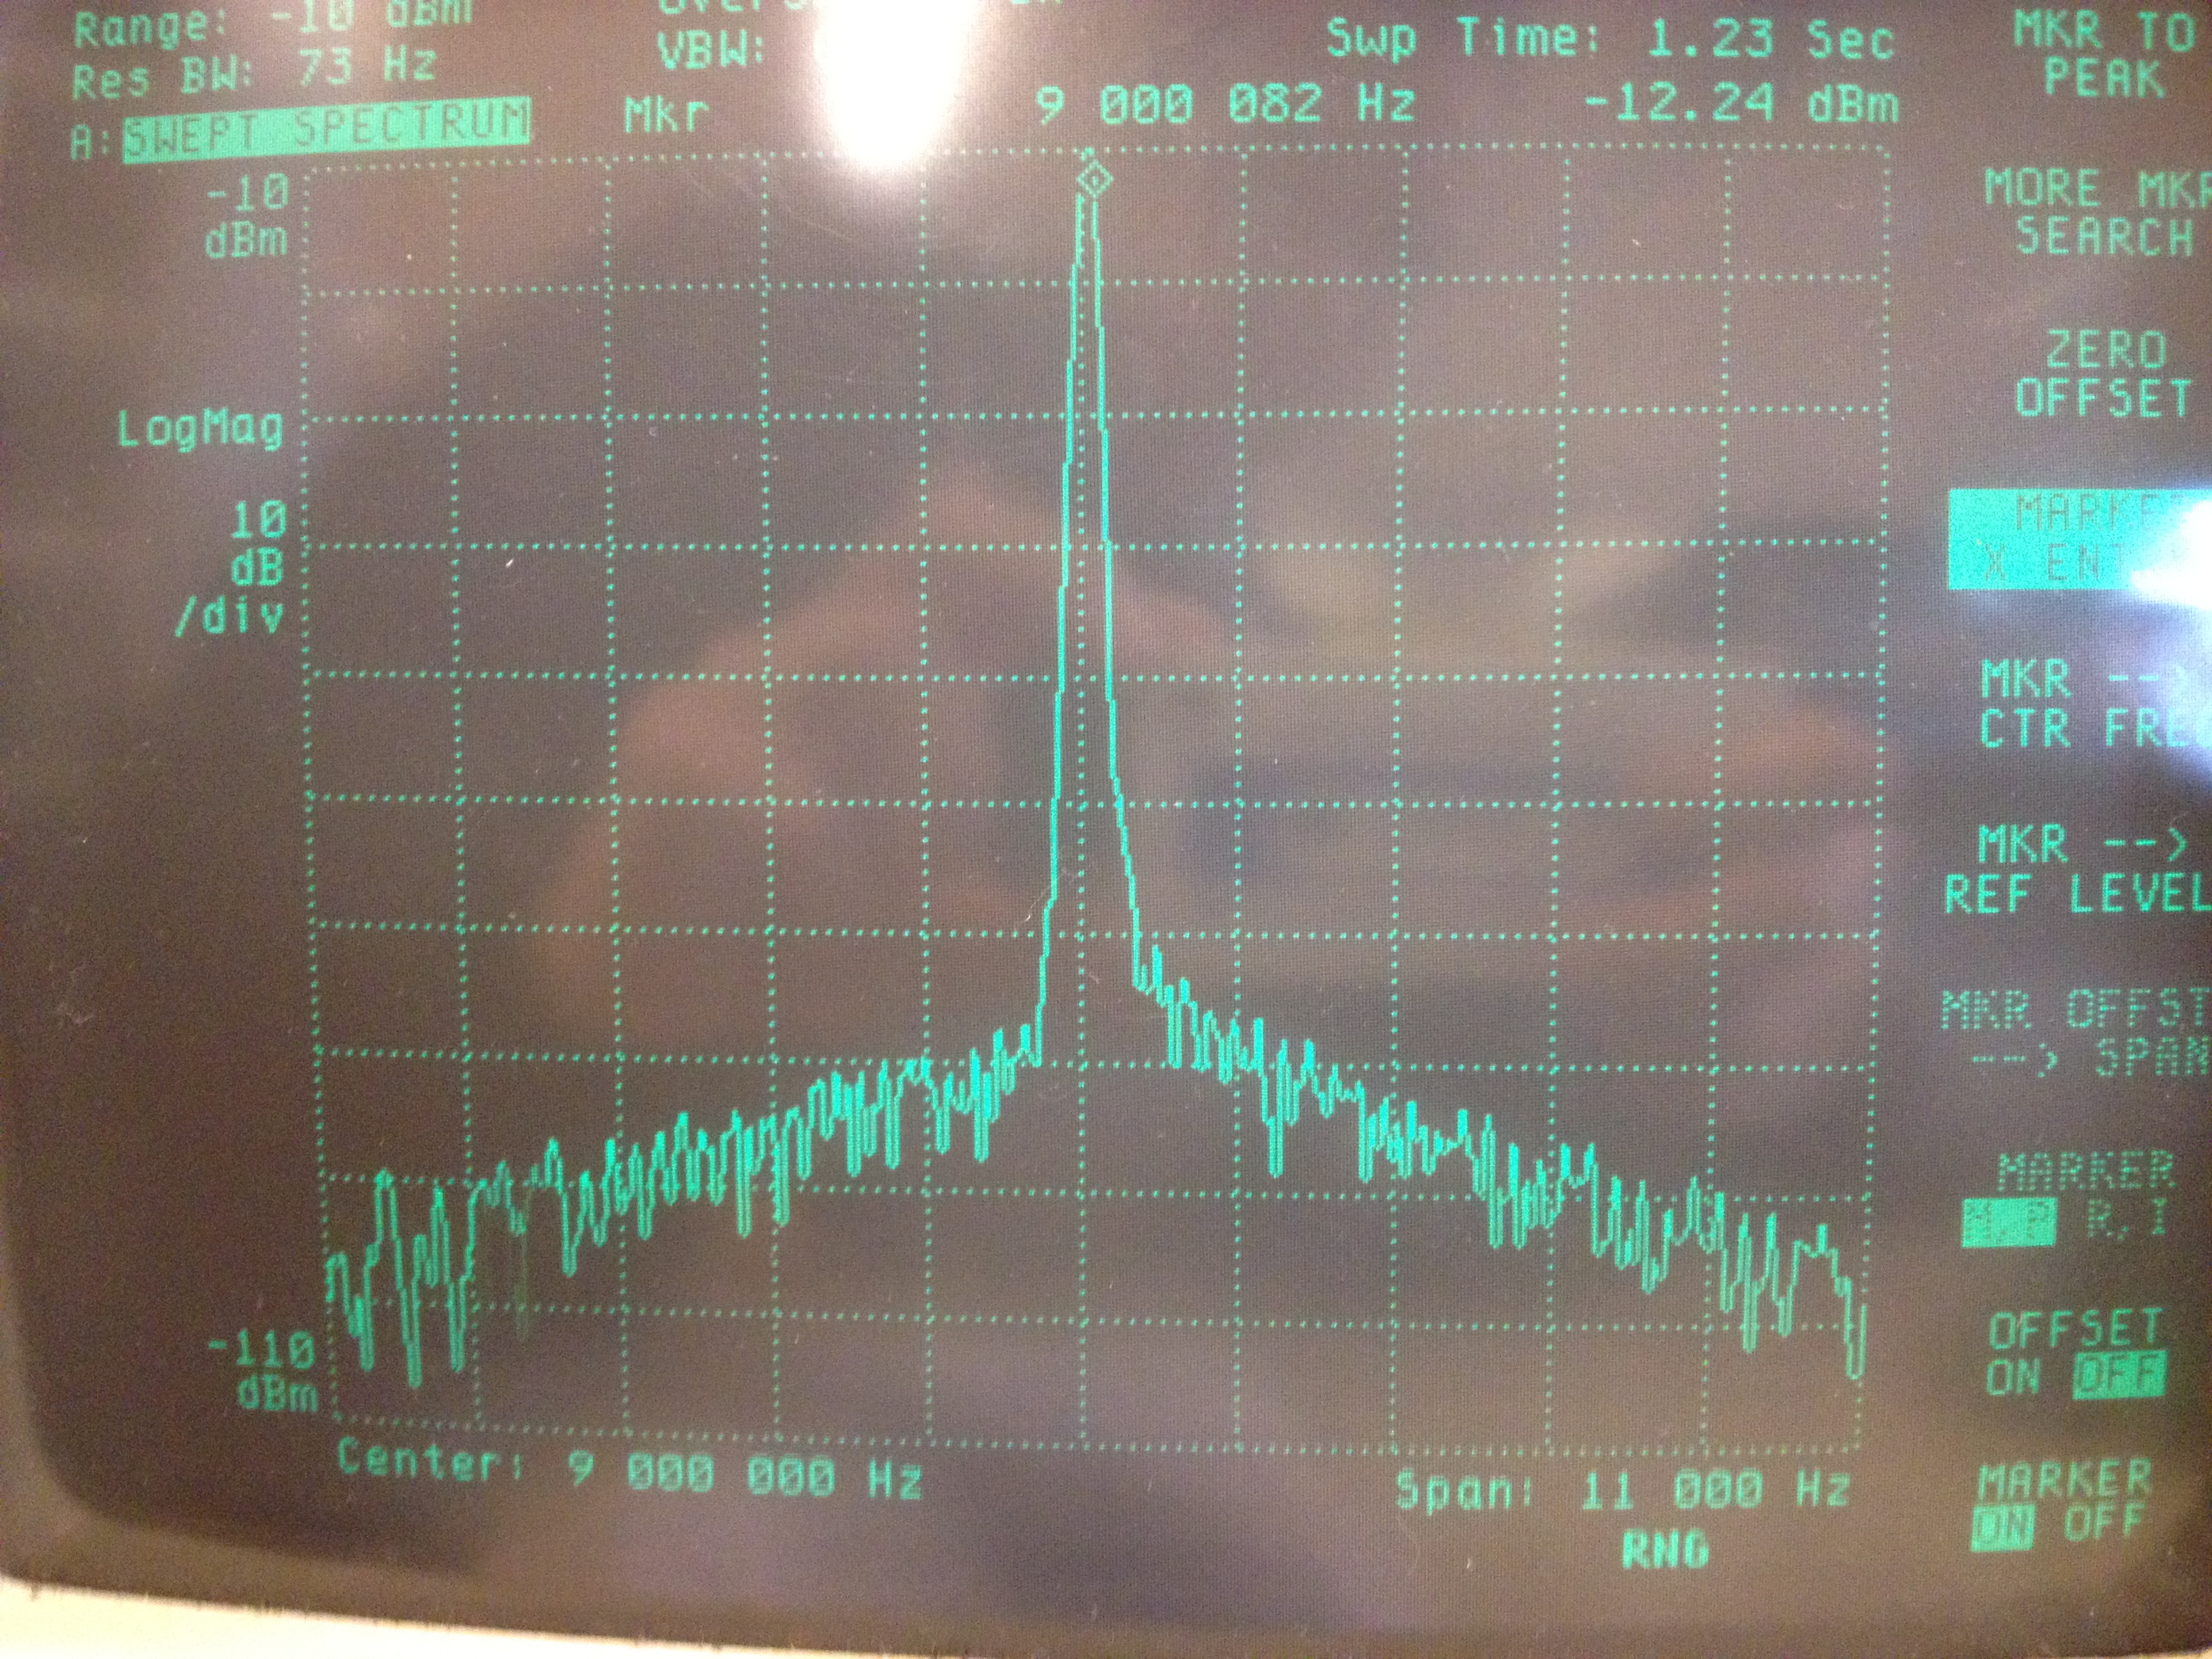
\includegraphics[width = 0.7\linewidth]{7_3_3_spectre9MHz.jpg}
\end{center}

Réglage de P41 : On constate que, lorsqu'on monte le curseur, la fréquence augmente. Augmenter le curseur revient à charger plus la sortie donc à diminuer le facteur de qualité du résonateur de sortie. Apparement notre quartz à une fréquence propre un peu plus élevée que 9MHz mais le réglage à été établi de manière à ajuster la fréquence. Le fait de diminuer le facteur de qualité diminue l'influence du réglage sur la fréquence, d'où un raprochement à la fréquence propre du quartz c'est à dire une augmentation.\\

Spectre de sortie de 1MHz à 100MHz :\\
\begin{center}
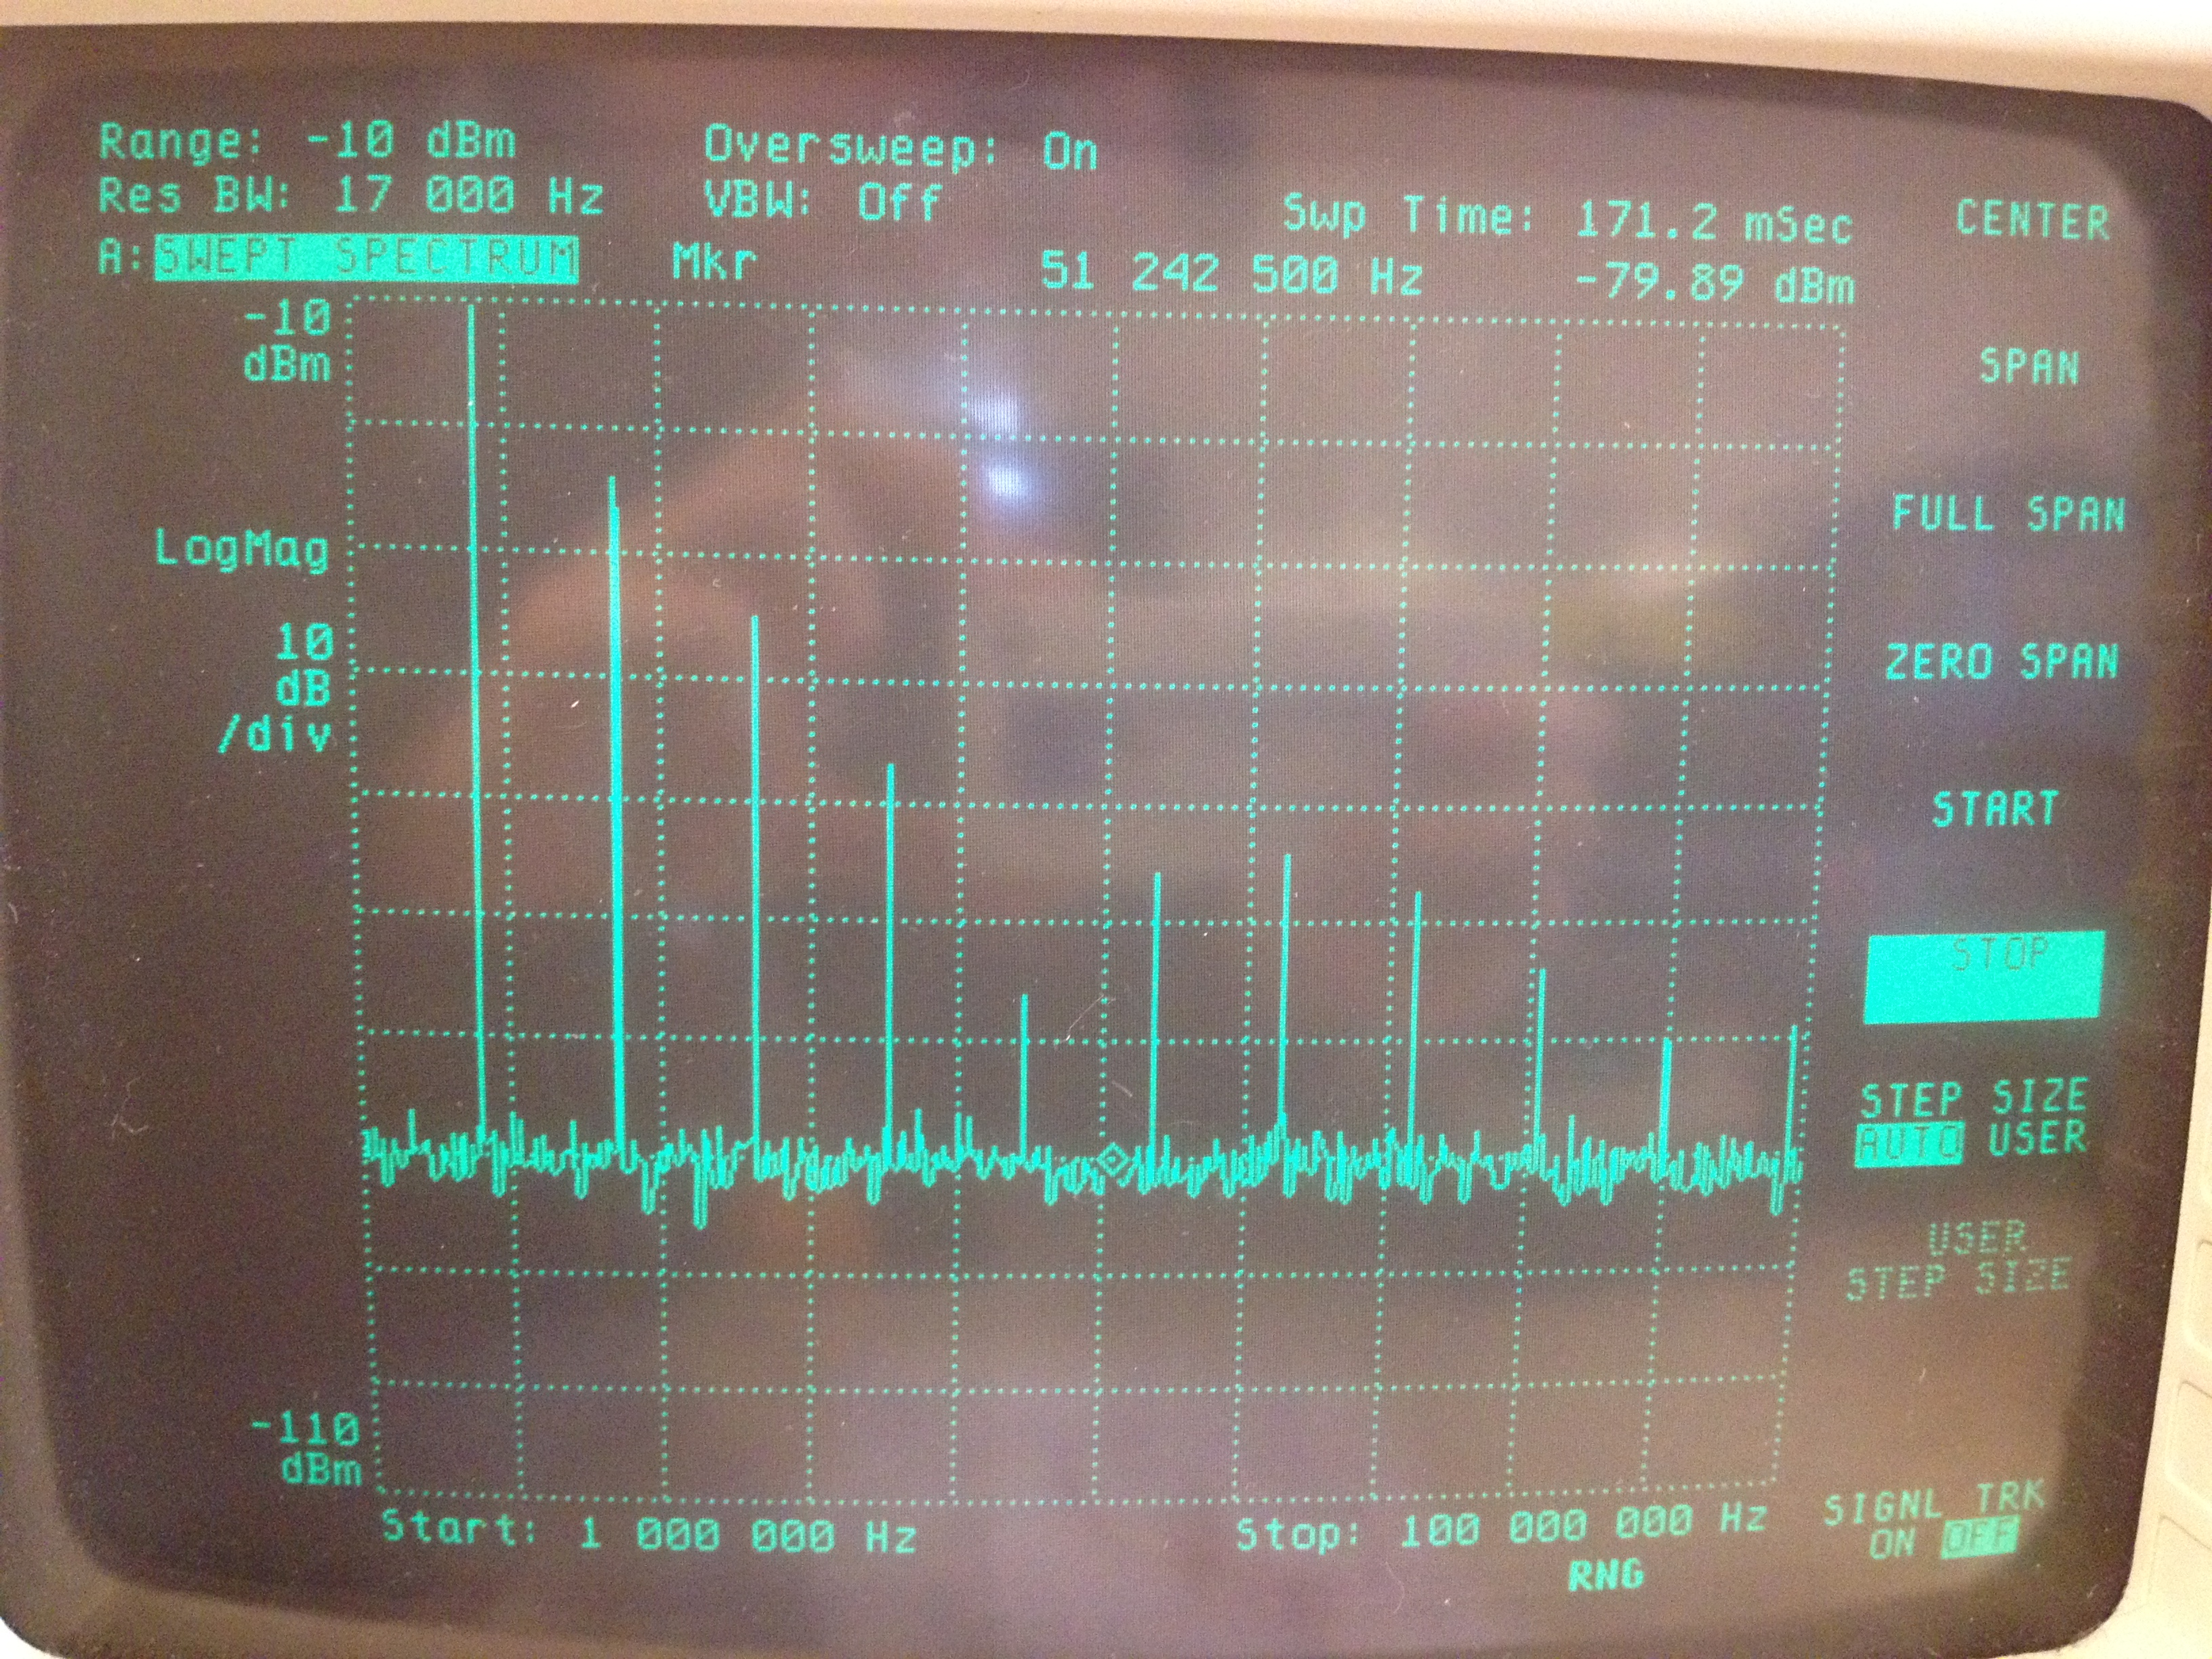
\includegraphics[width = 0.7\linewidth]{7_3_6_1MHz_100MHz.jpg}
\end{center}

On constate que le quartz à de nombreuses harmoniques, qui s'observent sur la sortie malgré le filtre de sortie $L_{41}$ et $C_{42}$. Sans l'effet de ce filtre, l'intensité de toutes les harmoniques serait probablement presque égal. Il est donc possible de faire osciller ce circuit à une autre fréquence avec le même quartz, en changeant les composants. On peut alors choisir une harmonique sur laquelle on vient s'accorder avec le quartz : Le filtre LC donne une grossière approximation de la région où les oscillations vont démarrer tandis que le quartz règle précisément la fréquence.


\section{Mélangeurs}

\subsection{Introduction}
Les mélangeurs sont des circuits qui permettent de multiplier deux signaux sinusoïdaux.
D'après la formule d'addition des sinus :
\begin{center}
$\sin(\omega_{1}\cdot t)\cdot \sin(\omega_{2}\cdot t) = \frac{1}{2}\cdot(\cos((\omega_{1} - \omega_{2})\cdot t) - cos((\omega_{1} + \omega_{2})\cdot t ) )$
\end{center}

Pour un montage idéal, nous avons donc une première composante fréquentielle en $\omega_{1} - \omega_{2}$ et une deuxième en $\omega_{1} + \omega_{2}$

Il est alors possible par filtrage d'éliminer l'une de ces deux composantes, typiquement $\omega_{1} - \omega_{2}$, afin de ne garder que la composante en $\omega_{1} + \omega_{2}$.\\

Ceci est utile pour réaliser plusieurs types de modulation et de démodulation.
\\
En pratique, la multiplication va présenter des non linéarités, nous aurons donc des harmoniques de $\omega_{1}$ et de $\omega_{2}$ en entrée du système.
Ainsi, nous avons des composantes à toutes les fréquences : $m \cdot \omega_{1} + n \cdot \omega_{2}$, $\forall m, n \in\bbZ$


\subsubsection{Mélangeur à circuit intégré NE602}

La multiplication des signaux IN1 et IN2 est faite par le circuit intégré NE602. 
Il s'agit d'un multiplicateur à 4 quadrants, c'est à dire que la sortie est valable pour toutes les combinaisons possibles des signes des tensions IN1 et IN2 (+, +), (+, -), (-, +) et (-, -).
Il n'y a donc aucunement besoin de polariser les entrées avec une composante continue, d'où un montage très simple.\\

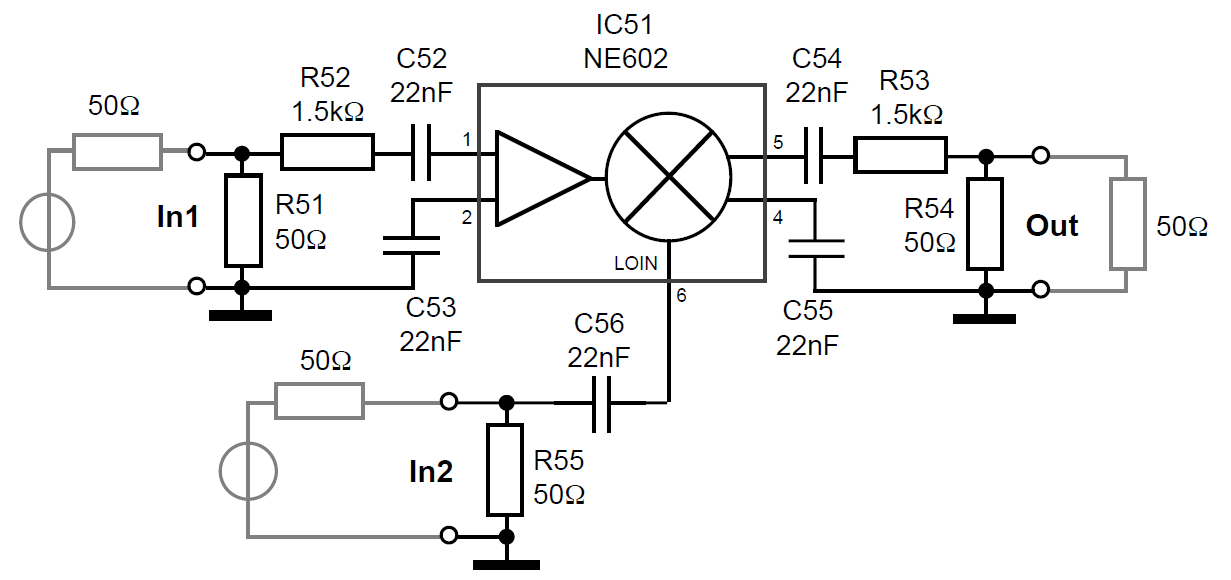
\includegraphics{shema_melangeur_gilbert.png}

L'impédance d'entrée sur l'amplificateur différentiel (broches 1 et 2) est d'environ $1.5k\Omega$ \footnote{Voir datasheet du composant NE602}. Idem pour les sorties sur les broches 4 et 5.
Les résistances $R_{51}$, $R_{52}$, $R_{53}$ et $R_{54}$ servent à adapter l'impédance du câble d'antenne $50\Omega$ vers le circuit intégré.\\

\begin{center}
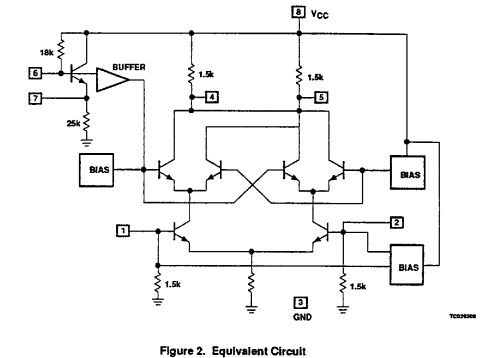
\includegraphics[width=0.85\linewidth]{shema_interne_ne602.png}
\end{center}

Le circuit à été prévu pour fabriquer un oscillateur avec les broches 6 et 7 cependant on n'utilise pas cette fonctionnalité, car nous avons notre propre oscillateur. L'amplitude doit être au moins de $200mV$ pour simuler un oscillateur local, qui n'est pas amplifié à l'intérieur du circuit, contrairement à l'entrée des broches 1 et 2 qui simule une antenne, et qui est amplifiée en interne.

Spectre de sortie :
\begin{center}
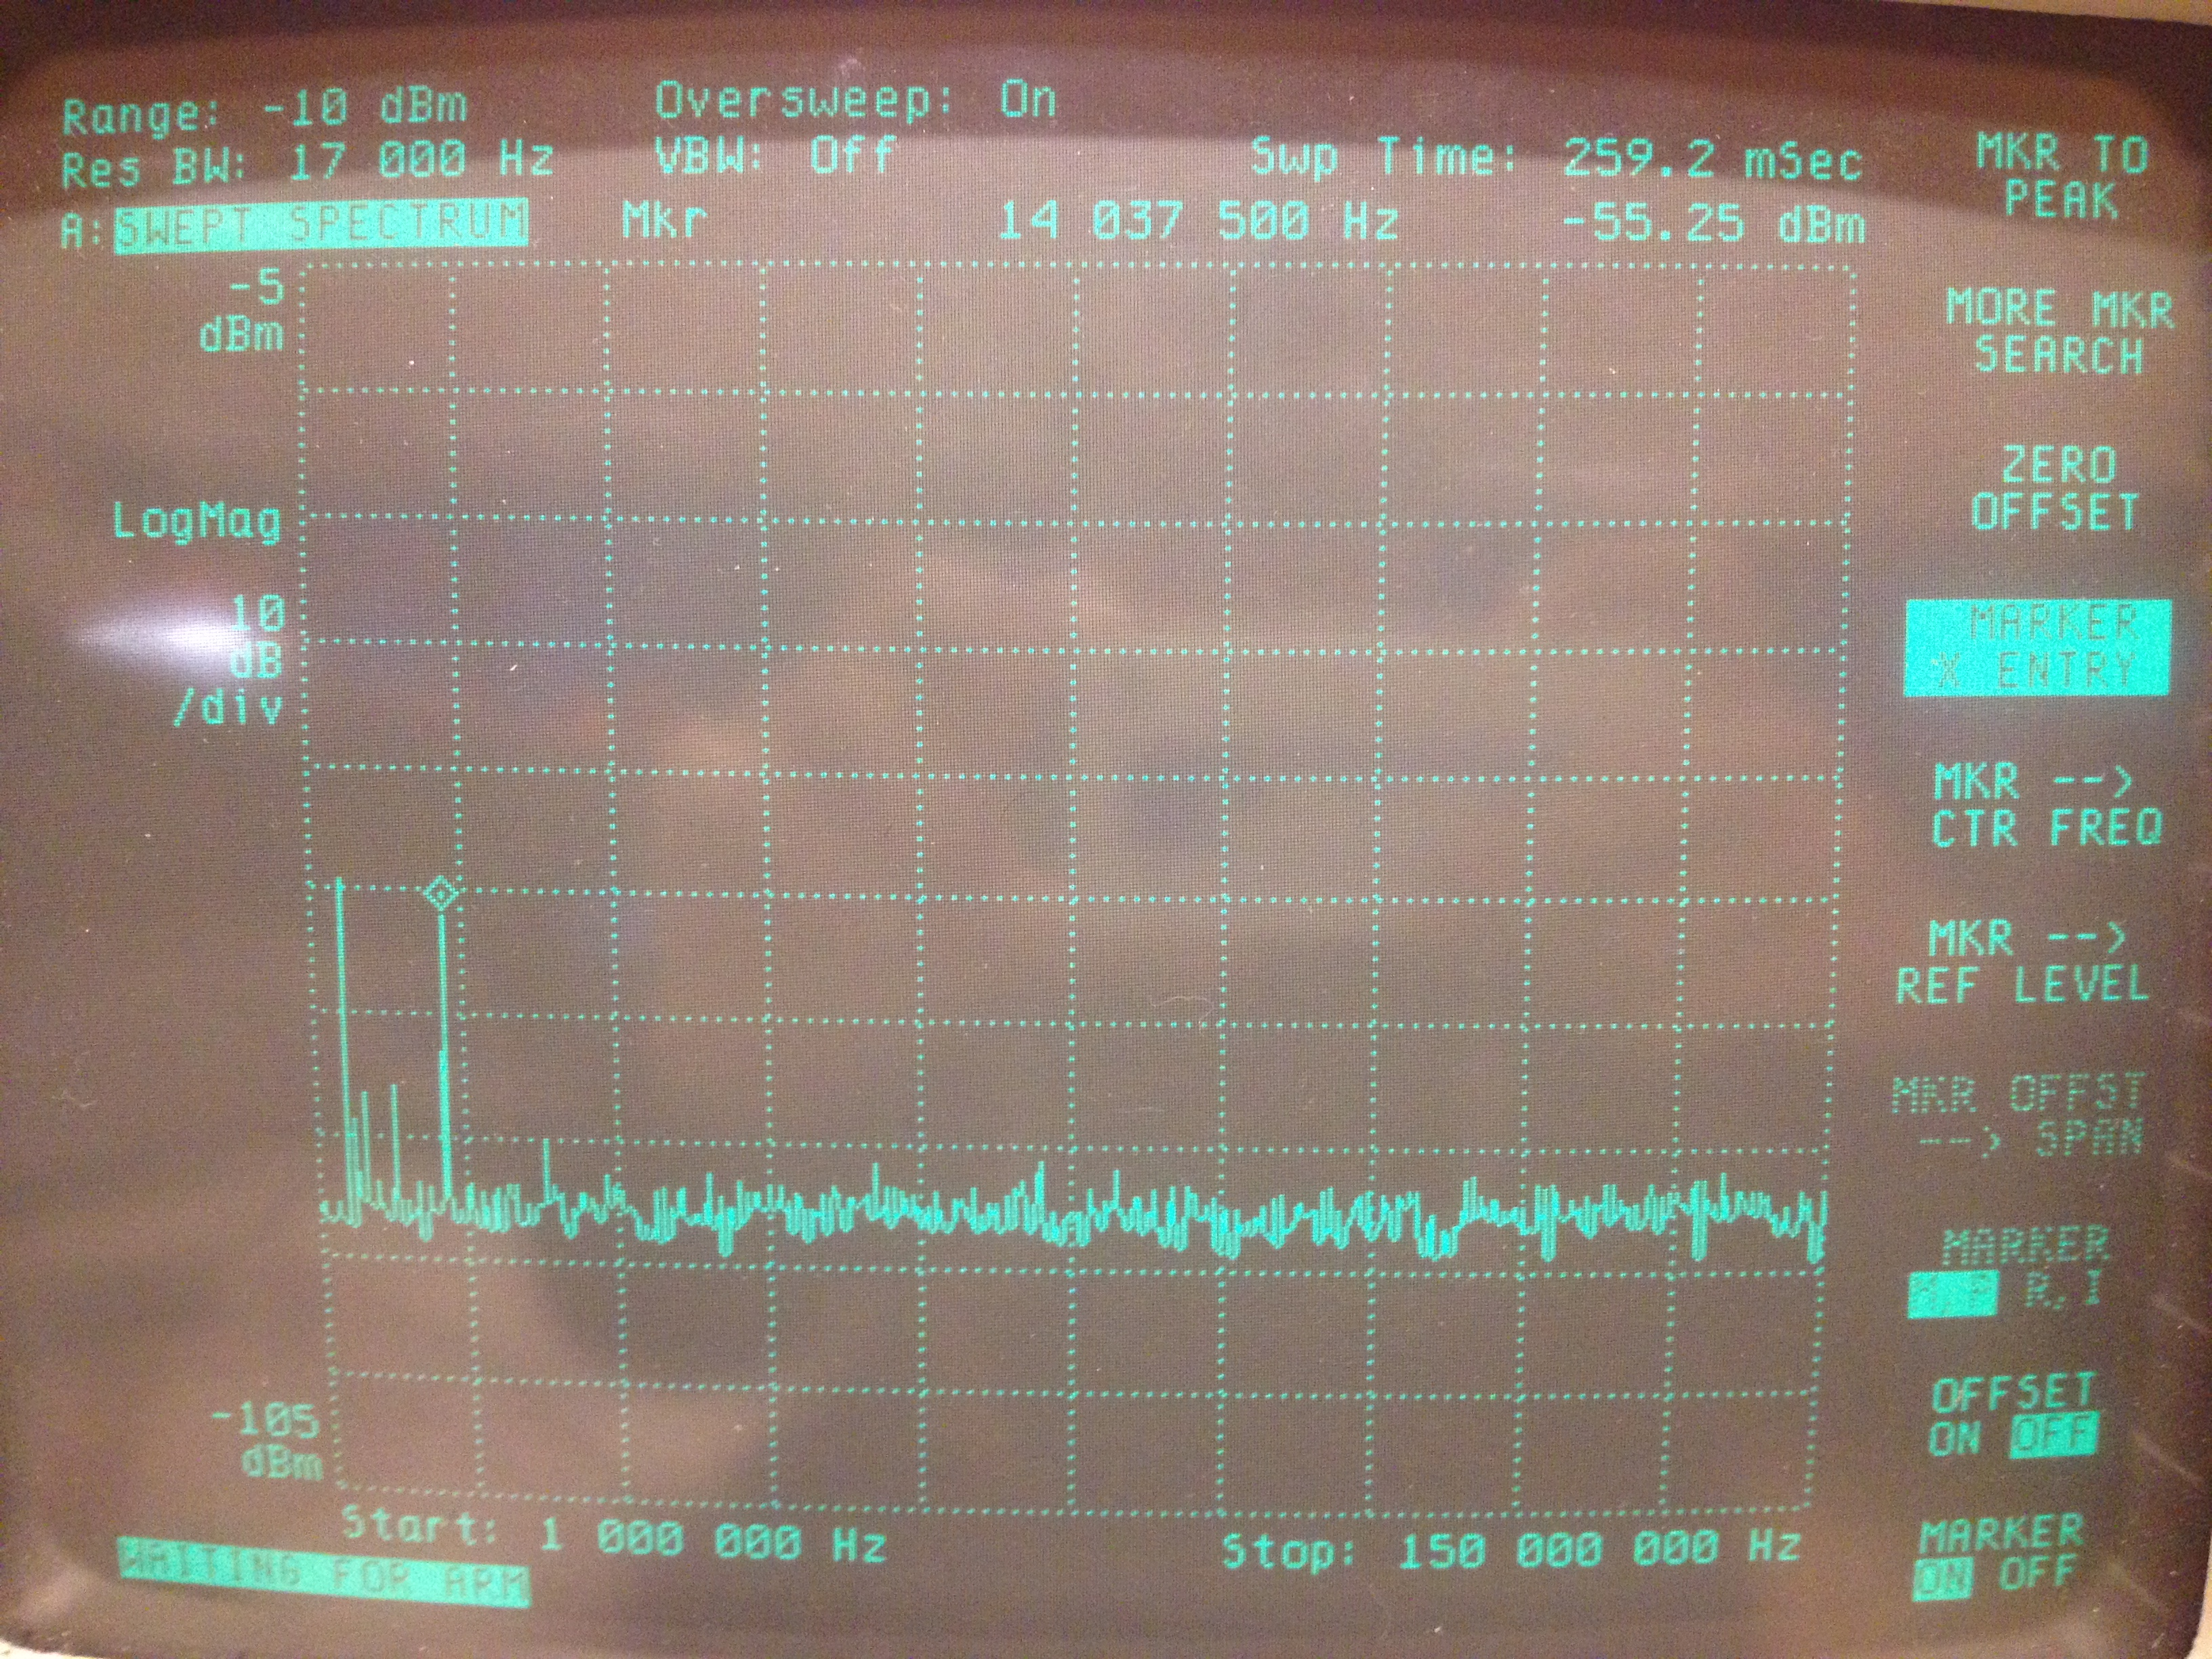
\includegraphics[width=0.7\linewidth]{8_3_1.jpg}
\end{center}
Mesures :
\begin{itemize}

\item Guain de conversion : 13.3 dB
\item Point de compression de 1dB : -8.2 dBm
\item Point d'interception du 3ème ordre : 6.55 dBm
\end{itemize}

A noter qu'il y a une perte de puissance considérable à cause du changement d'impédance. On perd la moitié du signal d'entrée utile sur le diviseur formé par $R_{in}$ et $R_{51}$, soit $-6$ dB. On perd une grande partie de la puissance de sortie à cause du diviseur formé par $R_{53}$ et $R_{54}$, les pertes sont de :
\begin{center}
$Pertes = 20\cdot \log (\frac{R_{54} // R_{out}}{(R_{54} // R_{out})+R_{53}}) = 20\cdot \log{25}{25+1500}) \simeq -35.7$ dB
\end{center}

Nous avons donc, en réalité, 41.7 dB de plus que ce que nous indique l'appareil.

Voici le spectre de sortie d'un signal double ton d'amplitude $-8$ dBm (l'appareil voit $-35.7$ dB de moins, soit $-43.7$ dBm):\\
\begin{center}
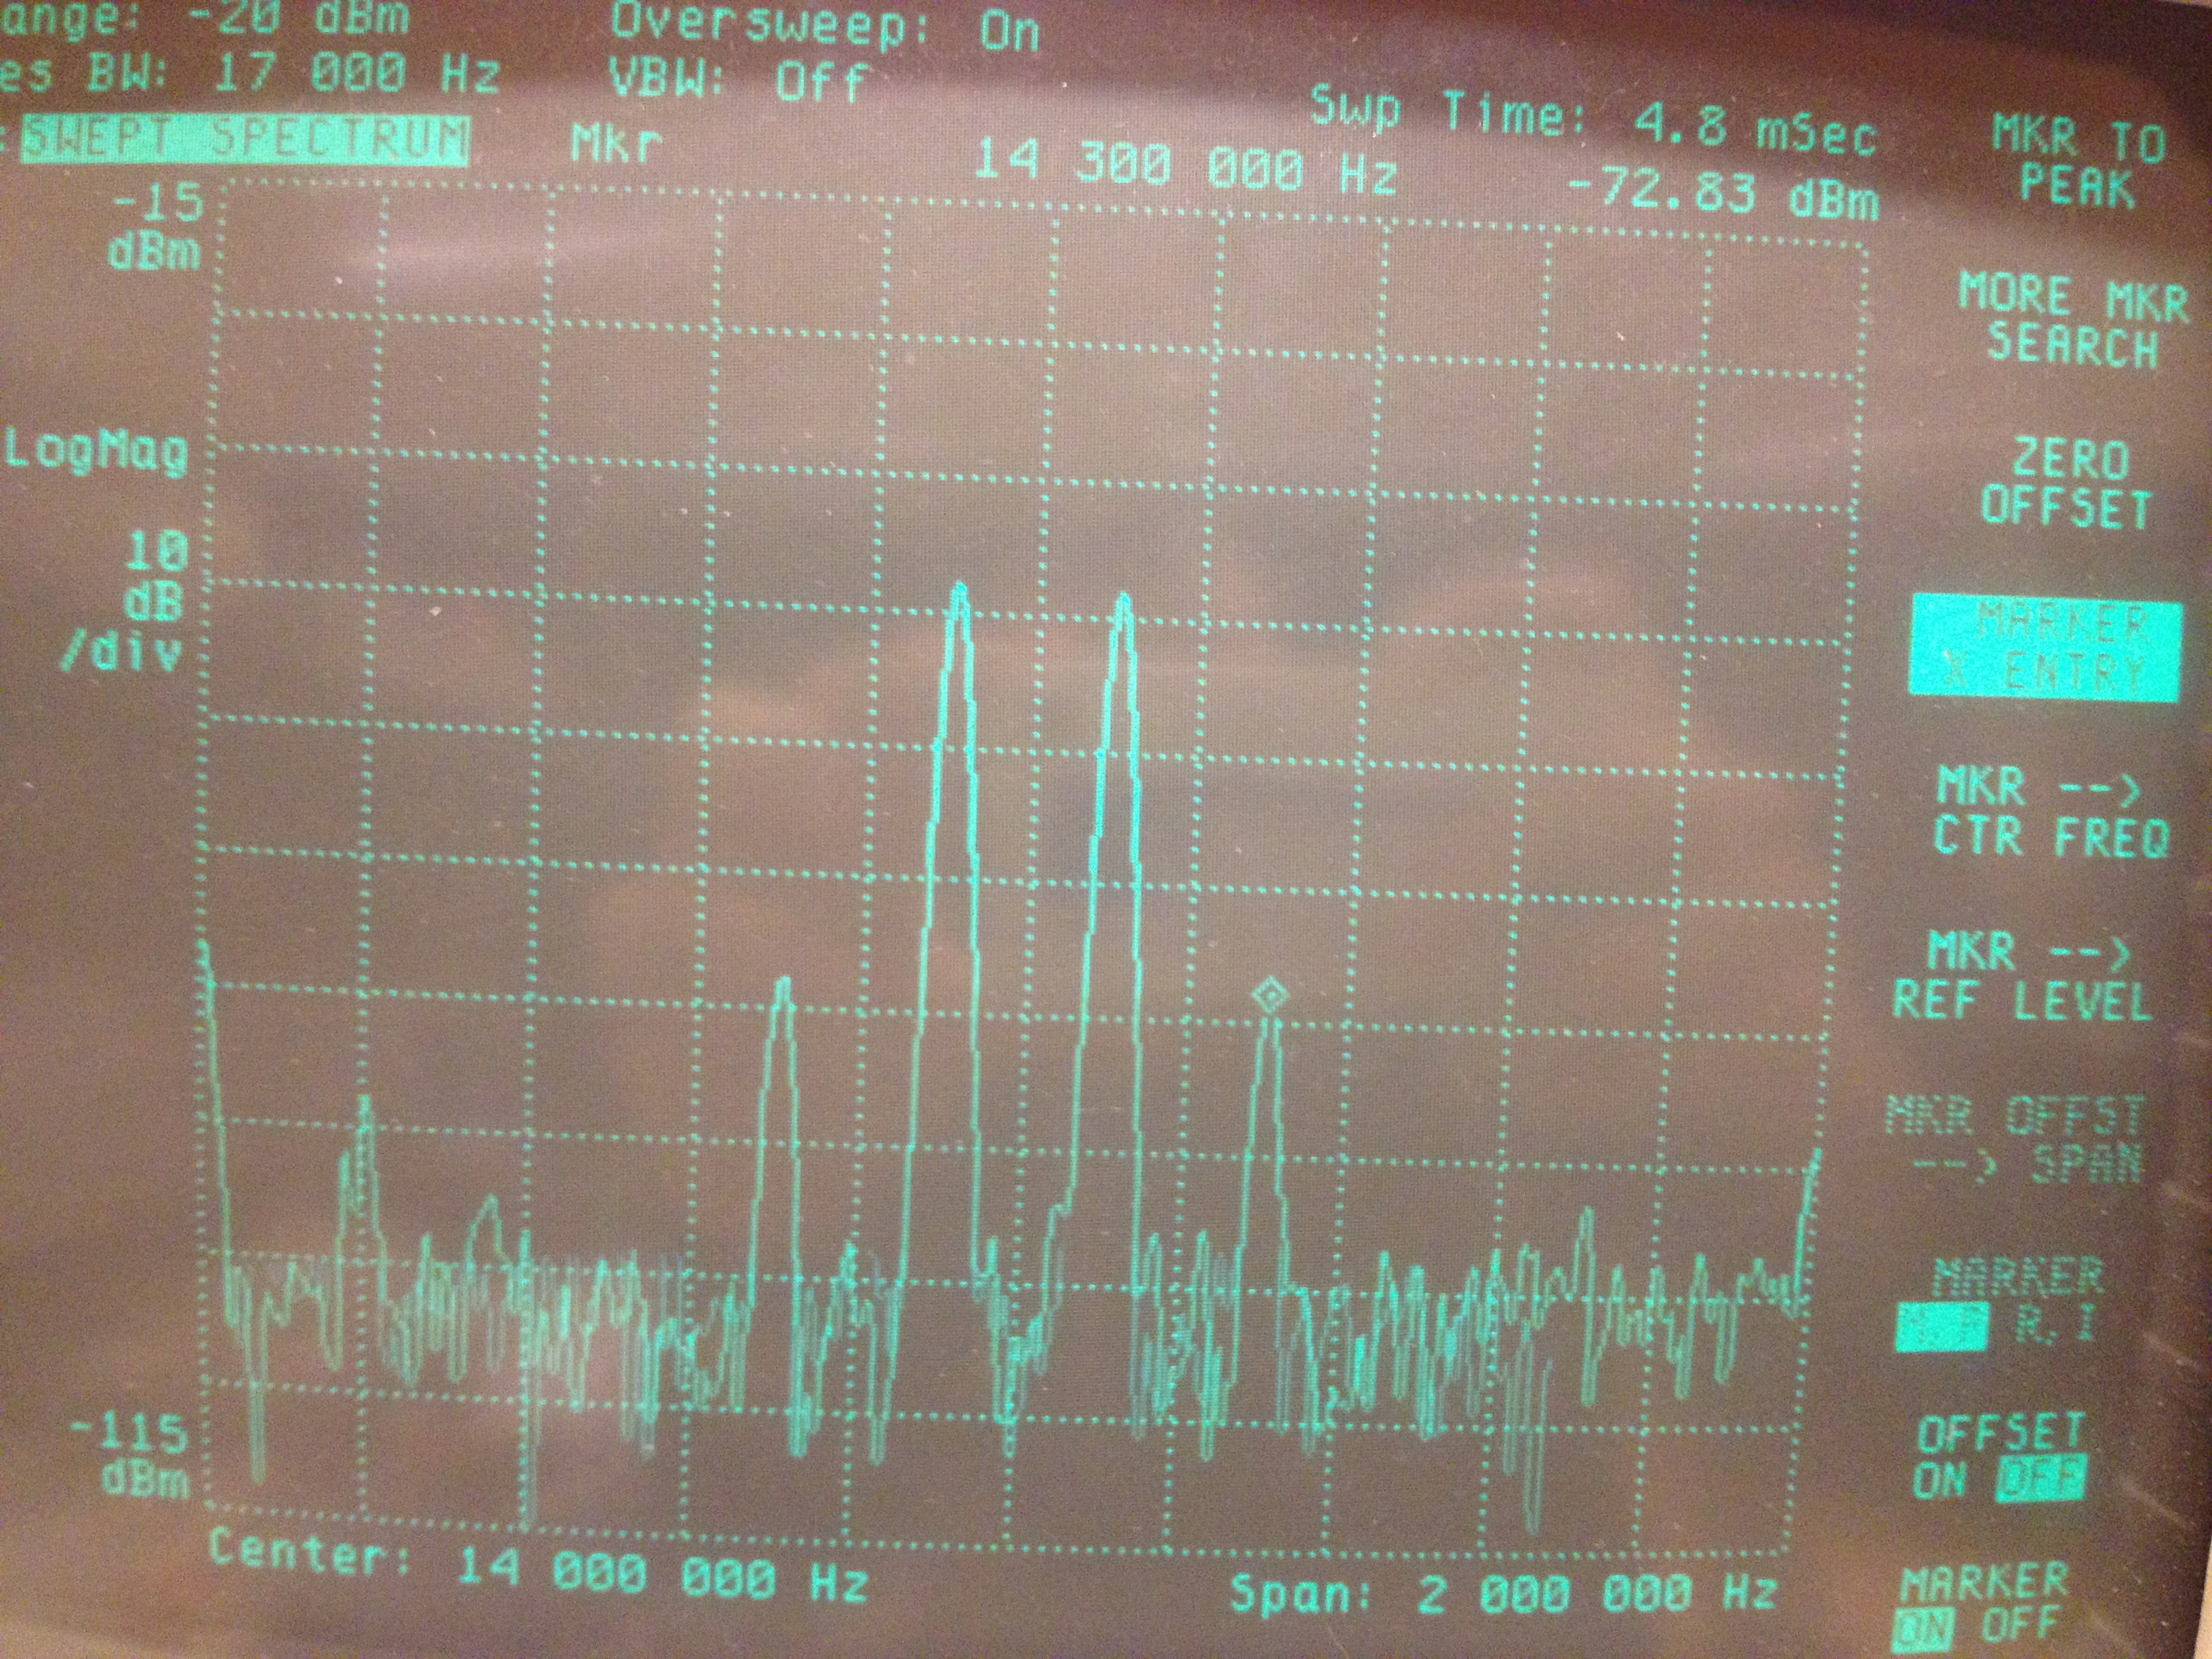
\includegraphics[width=0.7\linewidth]{8_3_4-8dbm.jpg}
\end{center}
Le pic de l'hamonique 3 est à $-72.8$ dBm pour l'appareil, c'est à dire en réalité $-72.8 + 35.7 = -37.1$ dBm.\\
On peut alors calculer le taux de distortion d'intermodulation d'ordre trois, c'est le point qui satisfait l'équation :
\begin{center}
$y = -37.1 + 3 \cdot (y+8) \Rightarrow y = 6.55$ dBm
\end{center}

% Est-ce vraiment correct ? Normalement on devrait être à -18 dBm (10 dB en dessous du point de compression, PAS à -8 dBm ?

%  9
%
%  In 9MHz = +7 dBm
%  In 5MHz = -7 dBm
%  Pic en sortie à 14MHz = -12.5 dBm
%  => Gain de conversion = -5.5 dB
%
%  In 5Mhz = 1 dBm  =>  Pic sortie 14MHz = -5.5 dBm, soit gain = -6.5 dBm
%  => Point de compression : In RF à 1dBm, soit 0.250 Veff
%
%  In1: 9MHz = 7 dBm
%  Out: 50.47 Ohm
%  In2: analyseur de spectre  =>  -58.5 dBm
%  =>  Gain = -67.5 dB
%


% 10
%
% On prend R77 = 560, R76 = 3.3k (on veut R76/R77=6)
% L72 pour fixer à 0 le potentiel moyen à G1 (sinon, on ne contrôle pas ce potentiel moyen). Comme ça, on peut polariser négativement blablabla G1.
%
% LO : 5MHz, 1Veff, 13.01 dBm
% RF : 9MHz, 10mVeff, -27dBm
% Sortie : plein d'harmoniques : multiples de 5MHz, de 9MHz, 9-k5 ...
% 14 MHz : -56.63 dBm
% Gain : -30.37 dB avec les réductions en entrée (Rin, R72) (-6dB) et en sortie (R73,R74,Rout) (-35.7 dB)
%    soit, sans ces adaptations : 11.33 dB
% Compression 1dB : In à -3.4 dBm, soit 0.151 Veff
%
% In2 : 5 MHz, 1 Veff
% IN1 : 9.1 MHz, 8.9 MHz, -5.4 dBm, 0.12 Veff
% => 14.3 MHz (3e harmo mesurée) : -70.9 dBm
%   (14.1 MHz : -42dBm)
%
% Avec 50.47ohm en sortie, IN2 avec 1Veff (13.01 dBm), l'analyseur sur IN1 :
% on mesure à 5MHz : -62.8 dBm
%  => -75.8 dB


% 11
%
% In1 : 10 mVeff, 9 MHz, -27 dBm
% In2 :  2 Veff,  5 Mhz, 19 dBm
% Sortie 14MHz : -80.1 dBm
% Gain : -53.1 dBm
% En prenant en compte les diviseurs de tensions internes : -11.4 dBm
% On réalise qu'en augmentant légèrement In1 à partir de 10mVeff, le gain augmente légèrement,
% avant de devenir constant pour une large gamme d'amplitudes pour In1.
% On fait donc les mesures de gain pour une amplitude de In1 légèrement supérieure à 10 mVeff :
% 20 mVeff
%
% in1 : 20 mVeff, -21 dBm
% Sortie 14MHz : -75 dbm
% Gain : -54 dBm
% En prenant en compte les diviseurs de tensions internes : -11.4 dBm
%
% In1 : 18.5 dBm  =>  Sortie 14MHz : -36.6 dBm
% = Gain de compression à -1dB
%
% In1 13.9 MHz, 14.1 MHz : 1.88 Veff, 18.5 dBM
% Sortie 14.3 MHz : -70.2 dBm
%









\end{document}